\documentclass[a4paper,10pt]{article}
\usepackage[utf8]{inputenc}
\usepackage{graphicx}
\usepackage{amsmath}
\usepackage{amssymb}
\usepackage{amsthm}
\usepackage{booktabs}
\usepackage{caption}
\usepackage{geometry}
%\usepackage{hyperref}
\usepackage{makeidx}
\usepackage{microtype}
\usepackage{subfig}
\usepackage{tabularx}
\usepackage{url}
\usepackage{varioref}
\usepackage{xcolor}
\usepackage{multicol}
\usepackage[italian]{babel}
\usepackage{mathtools}
\usepackage{booktabs}
\usepackage{multirow}
\usepackage{gensymb}


\addto\captionsenglish{
  \renewcommand{\contentsname}%
    {Indice}%
}



\title{Laboratorio I: Piano Inclinato\\ Misura dell'accelerazione attraverso sensori fotosensibili.\\
\begin{large}
Dipartimento di Fisica E.Fermi - Università di Pisa
\end{large}}

\author{Di Ubaldo Gabriele}
\date{11 Novembre 2015}

\begin{document}

\maketitle



%%%%%%%%%%%%%%%%%%%%%%%%%%%%%%%%%%%%%%%%%%%%%%%%%%%%%%%%%%%%%%%%%%%%%%%%%%%%%%%%%%%%%%%%%%%%%%%%%%%%%%%%%%%%%%%%%%%%%%%%%%%%%%%%%%%%%%%%%%%%%%%%%%%%%%%%%%%%%%%%%%%%%%%%%%%%%%%%%%%
\section{Introduzione}
\subsection{Teoria}
\textbf{Obiettivo:} Studiare il moto di diverse sferette su un piano inclinato e trovare le loro accelerazioni, usandole per stimare $g$ \\
La legge oraria che descrive il moto del centro di massa delle sfere è:
\begin{equation}
 s(t)=\frac{1}{2}at^2
\end{equation}
L'accelerazione di una sfera lungo il profilo inclinato è data da:
\begin{equation}
 a=\frac{5}{9}gsin\alpha
\end{equation}
\pagebreak

\subsection{Apparato sperimentale}
\begin{itemize}
\item{3 Sfere indicate con $S_i$}
\item{Un profilo mettallico ad angolo retto}
\item{Calcolatore con programma di acquisizione dati Plasduino}
\item{Due sensori ottici collegati al calcolatore}
\item{Calibro ventesimale di risoluzione $0.05mm$}
\item{Metro a nastro di risoluzione $1mm$}
\item{Livella elettronica}
\end{itemize}
Le sferette utilizzate sono indicizzate dalla più piccola alla più grande.

%%%%%%%%%%%%%%%%%%%%%%%%%%%%%%%%%%%%%%%%%%%%%%%%%%%%%%%%%%%%%%%%%%%%%%%%%%%%%%%%%%%%%%%%%%%%%%%%%%%%%%%%%%%%%%%%%%%%%%%%%%%%%%%%%%%%%%%%%%%%%%%%%%%%%%%%%%%%%%%%%%%%%%%%%%%%%%%%%%%
\section{Esperimento}
\subsection{Acquisizione misure}
Abbiamo misurato posto l'angolo $\alpha=3\degree$ con la livella elettronica. Dopodichè abbiamo scelto arbitrariamente 5 lunghezze cercando di esplorare il range più ampio possibile e rilevaond con i sensori i tempi di percorrenza per la sfera $S_1$ effettuando 5 misure per ogni lunghezza. 

Dopodichè  rilevato i tempi di percorrenza per le sfere $S_2$ ed $_3$ per verificare l'indipendeza dell'accelerazione dalle caratteristiche della sfera in questione.
Non è presente $v_0$ nell'equazione perchè abbiamo fatto in modo che fosse $v_0=0$ facendo partire le sferette da ferme e lasciandole libere esattamente prima di essere rilevate dal primo sensore cosicchè non potessero acquistare velocità.
Una fotocella è stata tenuta ferma per tutta la durata dell'esperimento e per variare la lunghezza abbiamo spostato solo la fotocella di partenza. Inoltre abbiamo mantenuto costante e uguale la distanza tra
il sensore e il profilo metallico nelle due fotocelle per evitare che la sfera fosse rilevata prima o dopo il dovuto.
 L'angolo misurato è la media dei valori trovati per diversi punti del profilo.
\begin{table}[!htb]
\centering
\caption{Sfera 1}
\label{my-label}
\begin{tabular}{c|ccccc|c}
$l(mm)$ & \multicolumn{5}{c}{$T(s)$}            & $T_m(s)$        \\ \hline
800     & 2.396 & 2.382 & 2.390 & 2.382 & 2.384 & $2.387\pm0.005$ \\
700     & 2.222 & 2.219 & 2.212 & 2.214 & 2.217 & $2.217\pm0.003$ \\
600     & 2.049 & 2.048 & 2.050 & 2.055 & 2.057 & $2.052\pm0.003$ \\
500     & 1.871 & 1.874 & 1.863 & 1.867 & 1.870 & $1.870\pm0.004$ \\
400     & 1.671 & 1.667 & 1.676 & 1.687 & 1.676 & $1.675\pm0.007$
\end{tabular}
\end{table}


\begin{table}[!htb]
\centering
\caption{Sfere 2 e 3}
\label{my-label}
\begin{tabular}{l|llllll}
$T-S_2(s)$ & 2.399 & 2.390 & 2.396 & 2.391 & 2.386 & $2.392\pm0.004$ \\ \hline
$T-S_3(s)$ & 2.346 & 2.354 & 2.346 & 2.348 & 2.352 & $2.349\pm0.003$
\end{tabular}
\end{table}


\subsection{Analisi dei dati}

Il seguente grafico descrive la relazione tra spazio percorso e periodo quadro:

 \begin{figure}[!htb]
\begin{center}
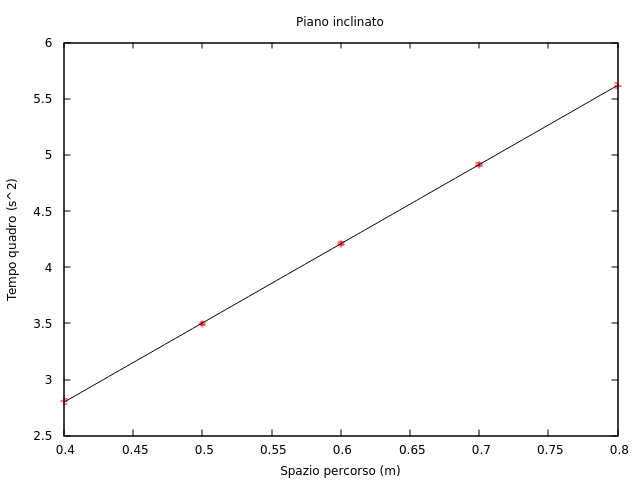
\includegraphics[width=10cm]{/home/zerch/Documents/UNIPI/LAB1/4Piano/grafici/graf-piano.png}
\end{center}
\end{figure}
I risultati del fit sono 
\begin{equation}
\chi2=5.45 \quad \chi2_r=1.81 \quad m=7.18\pm0.08 \quad b=-0.09\pm 0.05
\end{equation}
Dal coefficiente angolare $m$ possiamo stimare l'accelerazione della sfera, $m=2/a$, ottenendo $a=0.278\pm0.003m/s^2$. 
Da questo valore possiamo ottenre una stima di $g$. Il valore stimato è $g=9.56\pm0.1$


\section{Conclusione}
I dati convalidano il modello fisico per cui l'accelerazione è costante al variare lo spazio percorso e non dipende dalle caratteristiche della sfera come massa o volume. 
Il $\chi2$ conferma la validità della legge oraria. Il valore di $g$ non è compatibile con il valore noto probabilmente perchè il numero di misure è troppo basso.

%% valori corretti per i tempi 2.3687971631188689, 2.2158068507882178, 2.051438519673451, 1.8726985876002578, 1.6749925372968084

\end{document}


